% Graphic for TeX using PGF
% Title: C:\Documents and Settings\Admin\Мои документы\Мои рисунки\Диаграмма1.dia
% Creator: Dia v0.97.2
% CreationDate: Sat Sep 08 10:45:13 2012
% For: Admin
% \usepackage{tikz}
% The following commands are not supported in PSTricks at present
% We define them conditionally, so when they are implemented,
% this pgf file will use them.
\ifx\du\undefined
  \newlength{\du}
\fi
\setlength{\du}{15\unitlength}
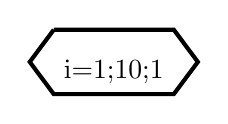
\begin{tikzpicture}
\pgftransformxscale{1.000000}
\pgftransformyscale{-1.000000}
\definecolor{dialinecolor}{rgb}{0.000000, 0.000000, 0.000000}
\pgfsetstrokecolor{dialinecolor}
\definecolor{dialinecolor}{rgb}{1.000000, 1.000000, 1.000000}
\pgfsetfillcolor{dialinecolor}
\pgfsetlinewidth{0.100000\du}
\pgfsetdash{}{0pt}
\pgfsetdash{}{0pt}
\pgfsetbuttcap
\pgfsetmiterjoin
\pgfsetlinewidth{0.100000\du}
\pgfsetbuttcap
\pgfsetmiterjoin
\pgfsetdash{}{0pt}
\definecolor{dialinecolor}{rgb}{1.000000, 1.000000, 1.000000}
\pgfsetfillcolor{dialinecolor}
\pgfpathmoveto{\pgfpoint{5.479214\du}{0.850000\du}}
\pgfpathlineto{\pgfpoint{8.371536\du}{0.850000\du}}
\pgfpathlineto{\pgfpoint{8.950000\du}{1.625000\du}}
\pgfpathlineto{\pgfpoint{8.371536\du}{2.400000\du}}
\pgfpathlineto{\pgfpoint{5.479214\du}{2.400000\du}}
\pgfpathlineto{\pgfpoint{4.900750\du}{1.625000\du}}
\pgfpathlineto{\pgfpoint{5.479214\du}{0.850000\du}}
\pgfusepath{fill}
\definecolor{dialinecolor}{rgb}{0.000000, 0.000000, 0.000000}
\pgfsetstrokecolor{dialinecolor}
\pgfpathmoveto{\pgfpoint{5.479214\du}{0.850000\du}}
\pgfpathlineto{\pgfpoint{8.371536\du}{0.850000\du}}
\pgfpathlineto{\pgfpoint{8.950000\du}{1.625000\du}}
\pgfpathlineto{\pgfpoint{8.371536\du}{2.400000\du}}
\pgfpathlineto{\pgfpoint{5.479214\du}{2.400000\du}}
\pgfpathlineto{\pgfpoint{4.900750\du}{1.625000\du}}
\pgfpathlineto{\pgfpoint{5.479214\du}{0.850000\du}}
\pgfusepath{stroke}
% setfont left to latex
\definecolor{dialinecolor}{rgb}{0.000000, 0.000000, 0.000000}
\pgfsetstrokecolor{dialinecolor}
\node at (6.925375\du,1.875000\du){i=1;10;1};
\end{tikzpicture}
